\documentclass{article}
\usepackage{graphicx}
\begin{document}
	\section*{Lsg Vorschlag RuTÜ07 Maximilian Maag}
	\section*{Aufgabe 7.1}
	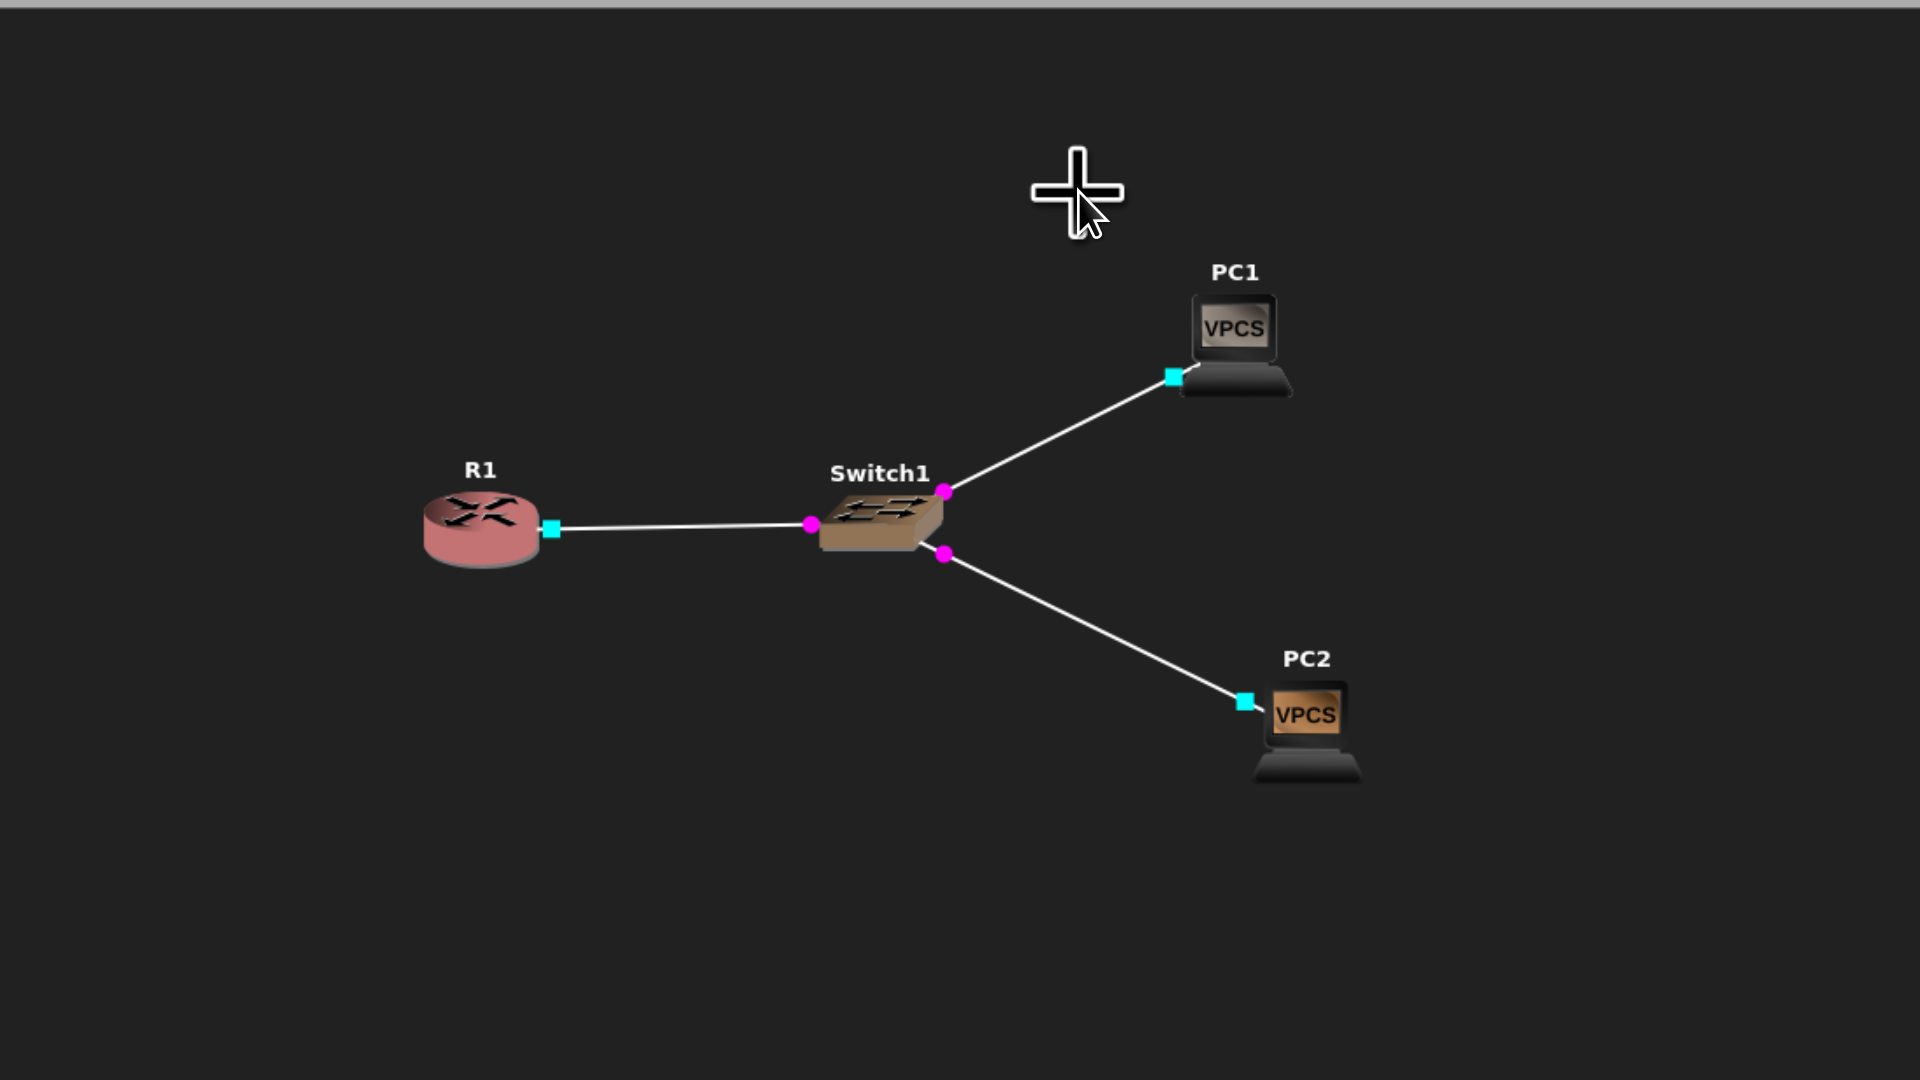
\includegraphics[width=\linewidth]{0701} \\
	Ohne Routing oder entsprechende Gateways können sich die PCs nicht gegenseitig anpingen.
	\section*{Aufgabe 7.2}
	Die entsprechenden IP Pakete werden vom Router über ein Routingprotokoll zwischen den entsprechenden Interfaces weitergereicht.
	\section*{Aufgabe 7.3}
	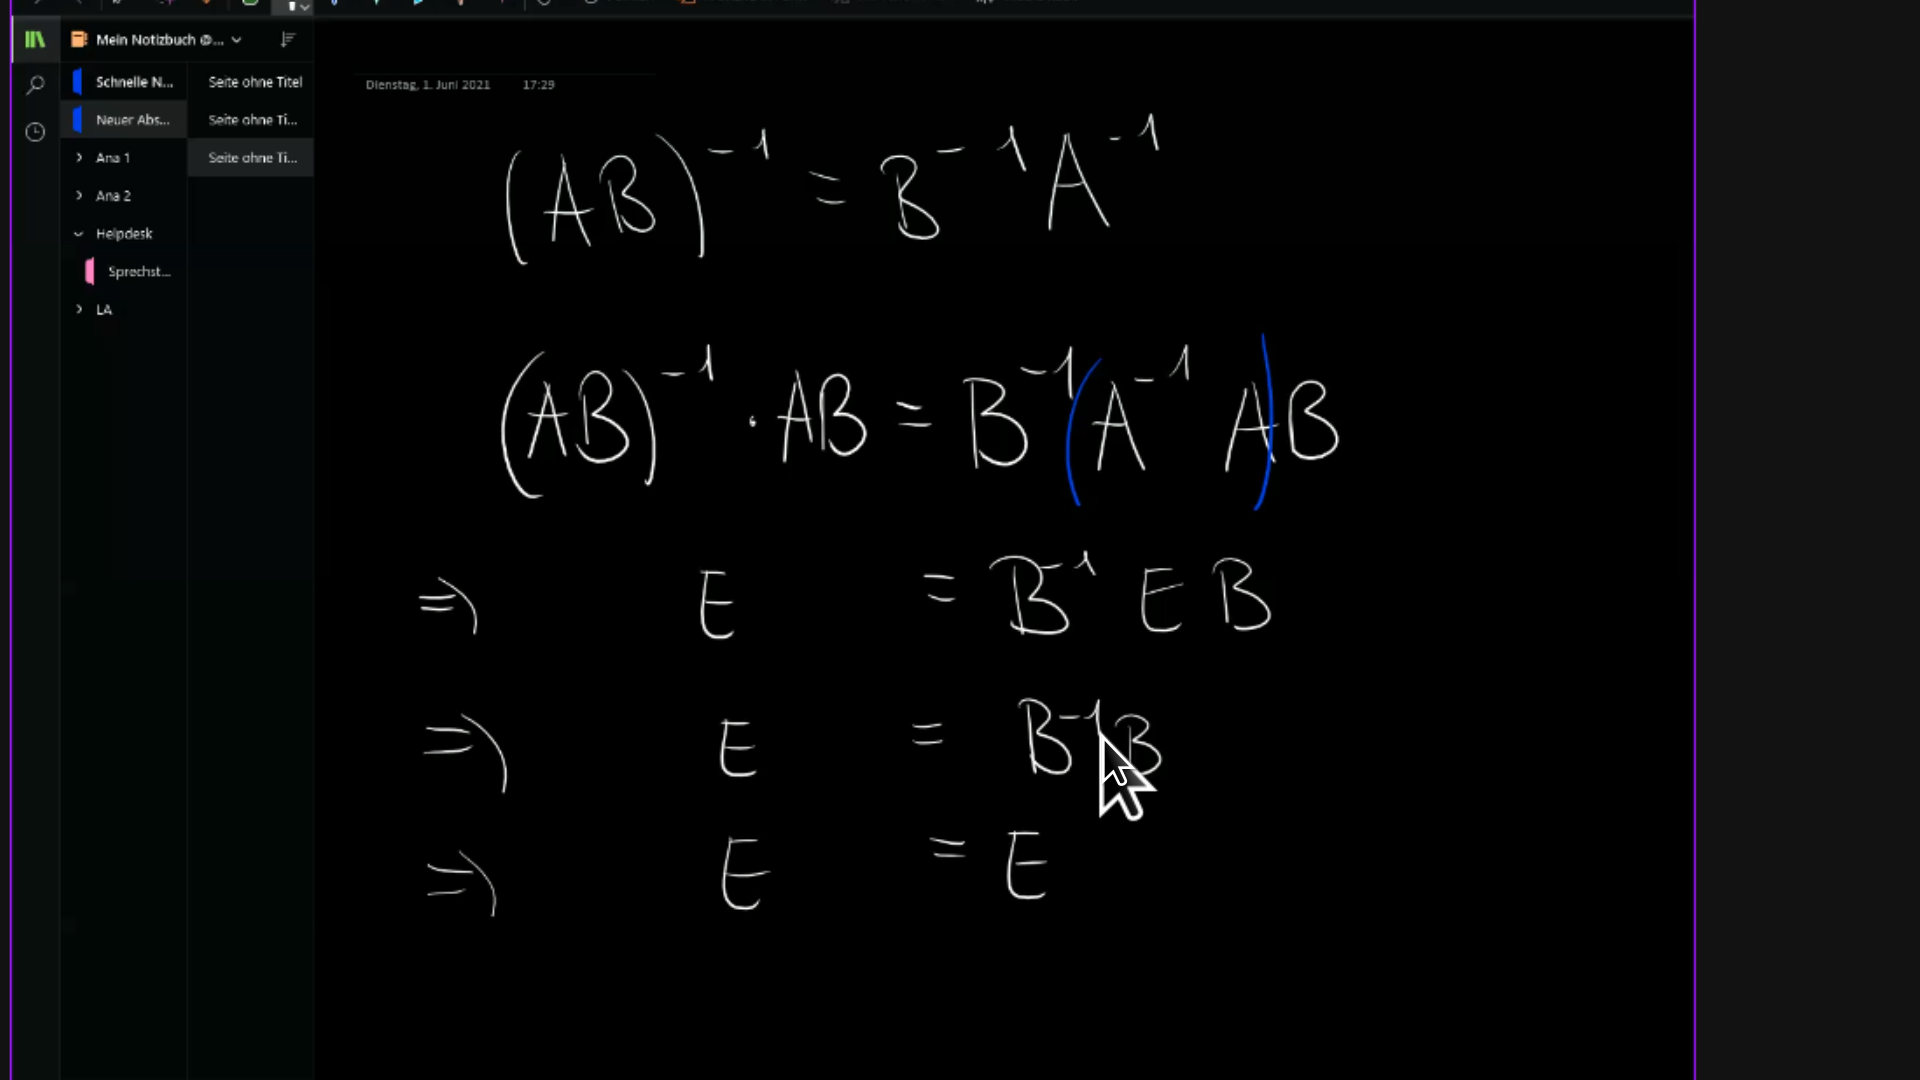
\includegraphics[width=\linewidth]{0703} \\
	Am Switch ist ein entsprechendes VLAN zu konfigurieren und am Router ist das Routing entsprechend des zusätzlichen VLANS zu erweitern.
	\section*{Aufgabe 7.4}
	Jeder Router kann seine direkten Nachbarn anpingen. Daraus ergibt sich folgende Konstellation: \\
	R1: R2 R4 \\
	R2: R1 R3 \\
	R3: R2 R4 \\
	R4: R1 Gateway
	\section*{Aufgabe 7.5}
	
	\section*{Aufgabe 7.6}
	Wenn das Interface abgeschaltet wird können Pakete zunächst nicht weitergeleitet werden bis über das DVC neue Ausweichrouten bekannt sind. Wiird das Interface wieder eingeschaltet wird es nach einem kurzen Updatezyklus wieder als Route erkannt und verwendet, entsprechend Distance Vector Routing.
\end{document}